\newcommand{\geomQuery}[2] {
  \null %emptyline
  \textbf{\uppercase{#1}} 
  \begin{adjustwidth}{2.5em}{0pt}
    #2
  \end{adjustwidth}
}

\chapter{Background}\label{ch:background}

\section{Monte Carlo Geometry Queries}

A Monte Carlo geometry kernel must be able to robustly support the types of
geometry queries

\geomQuery{Point Containment}{
    Given a volume and particle location, determine if the point is inside,
    outside, or on the boundary of that volume.
}

\geomQuery{Next Surface}{
  Given a volume, particle location, and particle trajectory, determine the next
  surface of the volume that the particle intersects along with the distance to
  that intersection.
}

\geomQuery{Closest Surface}{
  Given a volume and particle location, determine the distance to to the nearest
  surface of the volume in any direction.
}


\geomQuery{Surface Normal}{
  Given a surface and particle location, determine the normal vector of the
  surface at a point closest to the particle's location.
}

\geomQuery{Measure}{
    Given a volume or surface in the geometry, determine properties of that entity
  such as the volume or area.
}

\geomQuery{Next Volume}{
  Given a volume and surface, determine the adjacent volume on the other side of
  the surface.
}

\section{Analytic Geometry Representations}\label{sec:analytic_geometry}

This section contains a discussion of common analytic geometry  representations
which are often used in native representations of Monte Carlo geometry.

\subsection{Implicit Surfaces}\label{subsec:implicit_surfaces}

An implicit surface is a multivariate function defined over an $ R^3 $ domain as:

\begin{equation}
    \Omega(R^3)\rightarrow R
\end{equation}

Implicit surfaces are rich and versatile representation of closed manifolds used
for modeling, simulation, and rendering. Additionally, implicit surfaces can be
used to generate triangle meshes for rasterization or rendering on GPUs
\cite{Sethian_1996} and can also be constructed from arbitrary triangle meshes
or point clouds \cite{Sigg_2006}. Implicit surfaces are defined using the
isocontour of a scalar function defined over all space unlike an
\textit{explicit} representation of a surface which defines the subset of space
which the boundary occupies. Intuitively it might seem wasteful for a definition
to be true for all space considering the relatively small amount of space the
object will occupy, however a number of powerful tools for geometric modeling
using these representations will be discussed in this section.

An isocontour of this function with the value, $v$, can be described as:

\begin{equation}
  \Omega(\vec{x}) - v  = 0 
\end{equation}

For simplicity, the boundary of an implicit surface is defined as the isocontour
for which $v=0$. As a result, inside of the surface will have a negative value
while any point outside of the surface will have a positive value.

Unlike their explicit counterparts, implicit representations allow complex
topologies of surfaces to be integrated into a single representation. This is in
part because the function is defined for all space.As a result they handle the
merging and separation of disparate volumes well. These properties allow for
straightforward representation of dynamics surfaces such as fluids though this
is not of concern in the area of radiation transport. In practice, implicit
surfaces are used to extract mesh representations of surfaces, re-sample the
model into some other proxy for the geometry, and render models via ray
tracing. Implicit surfaces are well-suited to these applications due to the
integrated geometric properties that can be quickly recovered from their
analytic forms.

Important geometric information needed for visualization and simulation can be
readily recovered from implicit surface representations. For example, a common
operation in particle transport is the determination of its containment by a
volume in the model. A quick evaluation of the implicit function for this point
will indicate its containment by the sign of the function.
%% Such a process is more complex in the case of an explicit or discretized
%% representation. Typically this involves casting a ray through the model and
%% counting up the intersections or relying on the orientation of triangle normals
%% to indicate an entering or exiting intersection. The oddness or eveness of the
%% number of crossings will then determine the points containment.
Additionally, the distance to nearest intersection with the surface from any
point in space can quickly be determined via the definition of a signed distance
function, $d(\vec{x})$, formally defined as:

\begin{align}
  & d(\vec{x}) = min(|\vec{x} - \vec{x_{I}}|) \\
  & \Omega(\vec(x))  \,s.t.  \,|\Omega(\vec{x})| = d(\vec(x)) 
\end{align}

\begin{align}
  d \, &- \, signed \, distance \, function \\
  \vec{x_{I}} \, &- \,nearest \, boundary \,intersection
\end{align}

\noindent
Meaning that implicit surface functions can be modified to meet the three
requirements of a signed distance function:

\begin{figure}[H]
  \begin{center}
    \begin{minipage}{.8\textwidth}
      \begin{itemize}
      \item $ \Omega(\vec{x}) = d(\vec{x}) = 0 $ for all $x$ on the surface boundary
      \item $ \Omega(\vec{x}) = -d(\vec{x}) $ for all $x$ inside the surface boundary
      \item $ \Omega(\vec{x}) = d(\vec{x}) $ for all $x$ outside the surface boundary
      \end{itemize}
    \end{minipage}
  \end{center}
\end{figure}

Implicit surfaces are often used in time-dependent simulations due to their
natural extension into a fourth dimension ($ \Omega(\vec{x},t) - v  = 0 $) and
thus their support for moving boundaries and changing topologies. Implicit
surfaces are often broken up and represented by groups of Boundary
REPresentations (BREP's). 

\subsection{Constructive Solid Geometry}\label{subsec:csg}

Native Monte Carlo geometries are commonly formed from a standard set of
well-behaved implicit surfaces known as general quadratics. These surfaces are
then combined through Boolean operations to form more complex objects (as shown
in Figure \ref{fig:csg_ex}).

\begin{figure}[h]
  \centering
  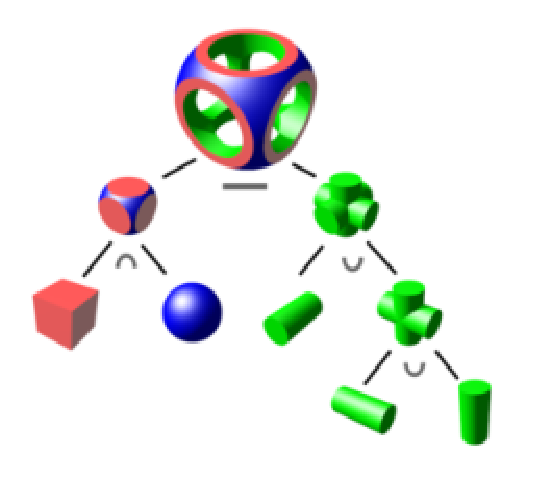
\includegraphics{csg_ex.eps}
  \caption{An example of how CSG volumes are created using Boolean combinations
    of smaller objects. The union of the three orthogonal cylinders is
    subtracted from the intersection of the box and sphere on the left to form
    the final volume at the top of the figure.}
  \label{fig:csg_ex}
\end{figure}

It is possible to construct complex geometries using CSG, but, as mentioned in
the introduction, the interface for this work is typically text-based and
defining complex volumes is a tedious and time-consuming task. Detecting
problems with the geometry definition is straightforward for the same reason
that particles can be robustly tracked through the geometry - the analytic
description of the surfaces. Fixing undefined regions of the geometry or
detecting invalid volume definitions is more difficult however.

The detection of intersections and particle containment queries in CSG
geometries is in practice computationally inexpensive for relatively simple
volume definitions, but due to the logical combinations of surfaces used to
create volumes the number of evaluations necessary to satisfy these queries is
linear with the number of surfaces in the definition. For sufficiently large and
complex models, it is not uncommon for volumes with many surfaces to be
artificially separated by planes to create two volumes with fewer surfaces in
their definition.

Visualization of CSG models can also be difficult. Because native formats for
CSG differ greatly between each Monte Carlo code, each typically comes with its
own visualization tools. These tools are typically restricted to 2D images of
the model representing a user-specified slice through the geometry. Other tools
such as MCAM \cite{Liu_2005} and McCad \cite{Tsigetamirat_2008} allow for
interactive visualization and repair of CSG models they do not provide the
accuracy of CAD modeling engines.

\subsection{CAD Geometry}

CAD systems allow for highly efficient and accurate geometric
representation. Highly complex models can be created using interactive
visualization tools represented in 3D space with a rich tool set for volume and
surface creation. These tools and the immediate visual verification of a user's
work reduces human error in model generation and design iteration.

In addition to reducing human error, CAD models provide a common domain for
analysis in other engineering domains such as fluid dynamics, heat transfer,
and structural engineering. This shared domain creates a common domain for
coupled physics simulation.

CAD also has the ability to represent free-form or higher-order surface. The use
of representations like splines and subdivision surfaces allow for more accurate
representation.

\subsection{Monte Carlo Radiation Transport on CAD Geometry}

The Direct Accelerated Geometry Monte Carlo (DAGMC) toolkit is a software
capable of Monte Carlo radiation transport directly on CAD models
\cite{Tautges_2009}. DAGMC was developed at the University of Wisconsin -
Madison. It has been coupled with many Monte Carlo codes to enable analysis on
CAD models. DAGMC relies on Cubit (and its commercial counterpart, Trelis) for CAD
modeling. Both of these CAD packages rely on the geometric modeling kernel,
ACIS.

DAGMC provides robust particle tracking for Monte Carlo transport on
arbitrarily complex CAD geometries. It accomplishes this by discretizing CAD
surfaces into sets of triangles. Volumes are then defined by any triangles which
represent bounding surfaces of a given volume. This surface mesh and the
geometric relationships between the mesh entities are stored in the Mesh
Oriented dAtaBase (MOAB) \cite{Tautges_2004}. These relationships are stored in
a hierarchical structure within MOAB, relating volumes to their surfaces,
surfaces to curves, and curves to vertices. 

It is important that geometric relationships of the mesh are maintained to
accelerate certain geometric queries on the surface mesh. For example,
\textit{Next Volume} queries are accelerated by using these relationships to
directly determine which volume a particle is passing into upon crossing a
surface rather than performing a query of the particle's location for each
volume. Other queries become more complicated due to the sheer number of
triangles needed to properly define volumes with detailed features. 

Next surface and closest to location geometry queries, for example, can be very
computationally expensive for volumes composed of hundreds of thousands or even
millions of triangles. A convenient way to think about performing geometric queries on
triangulated surfaces or volumes is to consider an equivalent CSG representation
constructed using a series of intersecting planes in place of triangles. The
structure imposed by the Boolean combinations used to define such volumes
require that each surface be checked for an intersection with the particle
trajectory. The nearest of these intersections can then be used to determine a
particle's crossing or movement to the physics event location specified by the
attached Monte Carlo code.

The problem of finding in intersection of a given particle location and
trajectory with a set of geometric primitives is known as ray tracing and is
well-studied in the field of computer graphics and animation. In this field,
data structures designed to accelerate the location of the nearest ray
intersection are applied.

\section{Ray Tracing Acceleration Data Structures}

Acceleration data structures for ray tracing are designed to rapidly narrow the
search for an intersection in virtual space given a starting position and
direction also known as a ray. This is accomplished by partitioning the space
and associating geometric primitives, most commonly triangles, with that
bounding partition. A search is performed by checking for an intersection with
the bounding partition. If the ray does not intersect with the partition, then
the set of primitives associated with that partition can be removed from the
search. If the ray does intersect with the partition, then the set of associated
primitives must be checked for intersection. Because a single separation into
two spatial partitions is often not enough to increase search efficiency, this
partitioning process is performed recursively. The result is a tree structure in
which at the top of the tree partitions are associated other partitions, known
as child nodes, rather than primitives. At the bottom of the tree exists a set of
nodes called leaves which are associated with geometric primitives. 

The search for a ray intersection then becomes a traversal of the tree
in which the children of the root node are checked for intersection. If an
intersection is found with one or both of the nodes, then the corresponding child nodes 
are checked for intersection as well. This process is repeated until leaf nodes
are reached at which point primitives are checked for intersection. Knowing that
a ray which doesn't intersect with a bounding partition cannot intersect with
any of the primitives it contains, allows many primitives to be rapidly removed
from the search and the number of intersection checks with primitives limited to
a small few. This technique reduces the algorithmic complexity of the search
from a brute force, or linear, $O(log(N_{triangles})$ to an $O(\,
log(N_{primitives}))$ search. 

\subsection{Partition Splitting Heuristics}

There are two components that go into the creation of spatial
partitions. The first is the selection of a candidate splitting plane which is
used to separate entities into one partition or another. The second is
the evaluation of the ``cost'' of that split should it be used. This cost is an
estimate of how good or bad the split would be. Because there is no way to know
exactly how expensive or inexpensive a split will be for the particular
simulation at hand, heuristics are used to evaluate this cost and determine the
optimal splitting plane using limited information about the local tree. This
information is typically limited to the number of primitives and bounds of the
parent partition and resulting child partitions.

The two heuristics will be addressed here - the Entity Ratio Heuristic (ERH) and the
Surface Area Heuristic (SAH). The ERH uses only the resulting number of
primitives in each child node to determine the cost of a split. The philosophy
behind this heuristic is to maintain the expected $O(log(N_{triangles})$ cost of
a ray traversal by ensuring that primitives are split as evenly as possible from
parent to child node. A form of this heuristic is presented in
Eq. \ref{eq:ERH}. This heuristic is unitless and bounded by zero and
one. This makes is possible to set both an upper and lower bound on the
unacceptable cost and a ``good enough'' cost.

\begin{figure}[H]
\begin{equation}
\label{eq:ERH}
 C = \frac{|P_{R}-P_{L}|}{(P_{R} + P_{L})} 
\end{equation}
  \begin{align*}
    C - & \,final \, cost \, evaluation \\
    P_{L} - & \, primitives\, contained\, by\, the\, left\, child  \\
    P_{R} - & \, primitives\, contained\, by\, the\, right\, child \\
  \end{align*}
  \caption{An example of the entity ratio calcution for a binary tree.}
  \label{fig:ERH}
\end{figure}

The SAH applies spatial information as well as division of primitives to the
cost evaluation. The SAH uses the surface area of candidate child partitions
relative to the current partition's surface area as an approximation for the
probability that the child will be visited after the parent volume. The explicit
form of the surface area heuristic was introduced in 1987 by Goldsmith and
Salmon \cite{Goldsmith_1987} and later formalized by MacDonald and Booth in 1990
\cite{MacDonald_1990}. Its full form is found in Equation \ref{eq:SAH}.

\begin{figure}[H]
  \begin{equation}
    C =  C_{t} + \frac{SA_{L}}{SA_{P}} |P_{L}|C_{i} +  \frac{SA_{R}}{SA_{P}} |P_{R}|C_{i}
    \label{eq:SAH}
  \end{equation}
  \begin{align*}
    C_{t} - & \,cost\, of\, traversal\, to\, child\, nodes \\
    C_{i} - & \, cost\, of\, primitive\, intersection\, check\, \\
    SA_{L} - &  \,surface\, area\, of\, left\, child \\
    P_{L} - & \, primitives\, contained\, by\, the\, left\, child  \\
    SA_{R} - & \, surface\, area\, of\, right\, child \\
    P_{R} - & \, primitives\, contained\, by\, the\, right\, child \\
    SA_{P} - & \, parent\, bounding\, volume \\
  \end{align*}
  \caption{A form of the surface area heuristic for a binary tree.}
  \label{fig:SAH}
\end{figure}

For the general case, ERH has not proved to be as effective as the SAH, but it
has proven to be a useful tool in correcting the surface area heuristic for
triangle mesh features of a specific type. This scenario will be discuss further
in <INSERT HV CHAPTER HERE>.
